\documentclass[a4paper]{article}
\usepackage[utf8]{inputenc}
\usepackage[russian,english]{babel}
\usepackage[T2A]{fontenc}
\usepackage[left=10mm, top=20mm, right=18mm, bottom=15mm, footskip=10mm]{geometry}
\usepackage{indentfirst}
\usepackage{amsmath,amssymb}
\usepackage{mathastext} 
\usepackage[italicdiff]{physics}
\usepackage{graphicx}
\usepackage{caption}
\usepackage{float}
\usepackage{caption}
\renewcommand{\thefootnote}{\fnsymbol{footnote}}
\usepackage{tablefootnote}
\usepackage{footmisc}
\usepackage{textcomp}
\usepackage{multicol}
\usepackage{multirow}
\usepackage[parfill]{parskip}
\usepackage{makecell}
\usepackage{array}  
\usepackage{siunitx}
\usepackage{booktabs}
\sisetup{
    exponent-product = \cdot,
    per-mode = symbol,
    separate-uncertainty = true,
    uncertainty-separator = \,
}
\renewcommand\cellalign{cc} 
\renewcommand\cellgape{\Gape[2pt]} 
\usepackage[utf8]{inputenc}\newcommand{\approxtext}[1]{\ensuremath{\stackrel{\text{#1}}{\approx}}}
\usepackage[colorlinks=true, urlcolor=blue, linkcolor=blue, citecolor=blue]{hyperref}
\graphicspath{{images/}}
\DeclareGraphicsExtensions{.pdf,.png,.jpg}
\usepackage{wrapfig}
\captionsetup{labelformat=empty}
\usepackage{caption}
\captionsetup[figure]{name=Рисунок}
\captionsetup[table]{name=Таблица}
%\usepackage{newtxtext,newtxmath} 
\title{\textbf{Отчет о выполнении лабораторной работы 4.7.2} \\[0.5em] \large\itshape Эффект Поккельса}
\date{}
\author{Котляров Михаил, Б01-402}

\begin{document}

\maketitle
	
\section{Введение}

\subsubsection*{Цель работы:} исследовать интерференцию рассеянного света, прошедшего кристалл; наблюдать изменение характера поляризации света при наложении на кристалл электрического поля.


\subsubsection*{Оборудование и инструментальные погрешности}

\textbf{Гелий-неоновый лазер "Плазма"}: длина волны любой модели $\lambda = 0,63$ мкм, погрешность не указана в документации,\\
\textbf{поляризатор},\\
\textbf{кристалл ниобата лития $LiNbO_3$}: размер 3x3x26 мм,\\
\textbf{матовая пластинка},\\
\textbf{экран},\\
\textbf{источник высоковольтного переменного и постоянного напряжения}: модель неизвестна,\\
\textbf{фотодиод},\\
\textbf{осциллограф GW Instek GOS-620},\\
\textbf{линейка}: цена деления 1 мм.\\


\section{Экспериментальная установка}

Схема экспериментальной установки представлена на рис.~\ref{fig:setup}. В качестве источника света используется гелий-неоновый лазер с длиной волны $\lambda = 0{,}63$~мкм. Излучение лазера линейно поляризовано в вертикальной плоскости. Для получения пучка лучей, падающих на кристалл под разными углами, перед кристаллом устанавливается матовая пластинка.

Основным элементом установки является кристалл ниобата лития (LiNbO$_3$), вырезанный вдоль оптической оси $z$. Размеры кристалла составляют $3 \times 3 \times 26$~мм. Кристалл помещён между двумя поляризационными элементами: входной поляризатор в данной работе не используется, поскольку излучение лазера уже поляризовано, а на выходе установлен анализатор (поляроид), пропускающий свет с горизонтальной поляризацией (скрещённые поляризации). За анализатором располагается экран, на который проецируется интерференционная картина. Расстояние от середины кристалла до экрана составляет $L$ = 70÷80~см (в зависимости от условий освещения).

Для исследования эффекта Поккельса на кристалл подаётся электрическое напряжение от источника высоковольтного постоянного или переменного напряжения. В качестве фотоприёмника используется фотодиод, сигнал с которого подаётся на $y$-вход осциллографа. На $x$-вход осциллографа подаётся напряжение, пропорциональное приложенному к кристаллу напряжению, что позволяет наблюдать фигуры Лиссажу.

\begin{figure}[h]
    \centering
    
\includegraphics[width=0.7\textwidth]{Pictures/setup.png}
    \caption{Рис. 1. Схема экспериментальной установки}
    \label{fig:setup}
\end{figure}

\section{Выполнение}

\subsection*{Юстировка системы}
Перед началом измерений проведём юстировку оптической схемы. Вначале без кристалла установим анализатор таким образом, чтобы лазерное излучение через него не проходило, то есть установим скрещенные поляризации. Для определения разрешённого направления анализатора используем отражение дневного света от горизонтальной поверхности; при вращении анализатора найдём минимум освещённости, что соответствует вертикальному разрешённому направлению. Затем поместим в оптическую схему кристалл ниобата лития, а перед ним вплотную к кювете установим матовую пластинку. Расстояние от кристалла до экрана выберем $L = 75,0 \pm 0,5$ см, что обеспечит чёткую интерференционную картину. Вращением юстировочного винта и поворотом рейтера с кюветой вокруг вертикальной оси добьёмся совмещения центра коноскопической картины с положением лазерного луча на экране. Повернём анализатор на $90^\circ$ и убедимся в изменении картины на негативную, после чего вернём анализатор в исходное положение (горизонтальное разрешённое направление).

\subsection*{Определение двулучепреломления кристалла}
Для определения разности показателей преломления $n_o - n_e$ измерим радиусы тёмных интерференционных колец. 

\begin{table}[h!]
\centering
\begin{tabular}{|c|c|}
\hline
№ & $D_1$, см \\
\hline
1 & 5,3 \\ \hline
2 & 5,2 \\ \hline
3 & 5,2 \\ \hline
\end{tabular}
\caption{Таблица 1. Измерения диаметра первого кольца}
\label{tab:ring1}
\end{table}

Исходя из первого измерения рассчитаем полную погрешность: $\sigma_\text{сист} = 0,1$ см, $\sigma_\text{случ} = 0,033$ см, \\$\sigma = \sqrt{\left( \sigma_\text{случ} \right)^2 + \left( \sigma_\text{сист} \right)^2} = 0,105$ см. Далее для всех колец берется именно эта погрешность.

\begin{table}[h!]
\centering
\begin{tabular}{|c|c|}
\hline
$m$ & $D$, см \\
\hline
1 & 5,23 \\ \hline
2 & 7,4 \\ \hline
3 & 9,2 \\ \hline
4 & 10,7 \\ \hline
5 & 11,6 \\ \hline
6 & 13,0 \\ \hline
7 & 14,2 \\ \hline
8 & 15,1 \\ \hline
\end{tabular}
\caption{Таблица 2. Результаты измерений диаметров интерференционных колец}
\label{tab:rings}
\end{table}

Для каждого кольца с номером $m$ измерим диаметр $D_m$, после чего вычислим радиус $r_m$ и его квадрат $r_m^2$. Построим график зависимости $r_m^2$ от номера кольца $m$ (рис.~\ref{fig:r2m}). Аппроксимируем экспериментальные точки прямой линией методом взвешенной регрессии.

\begin{figure}[h]
    \centering
    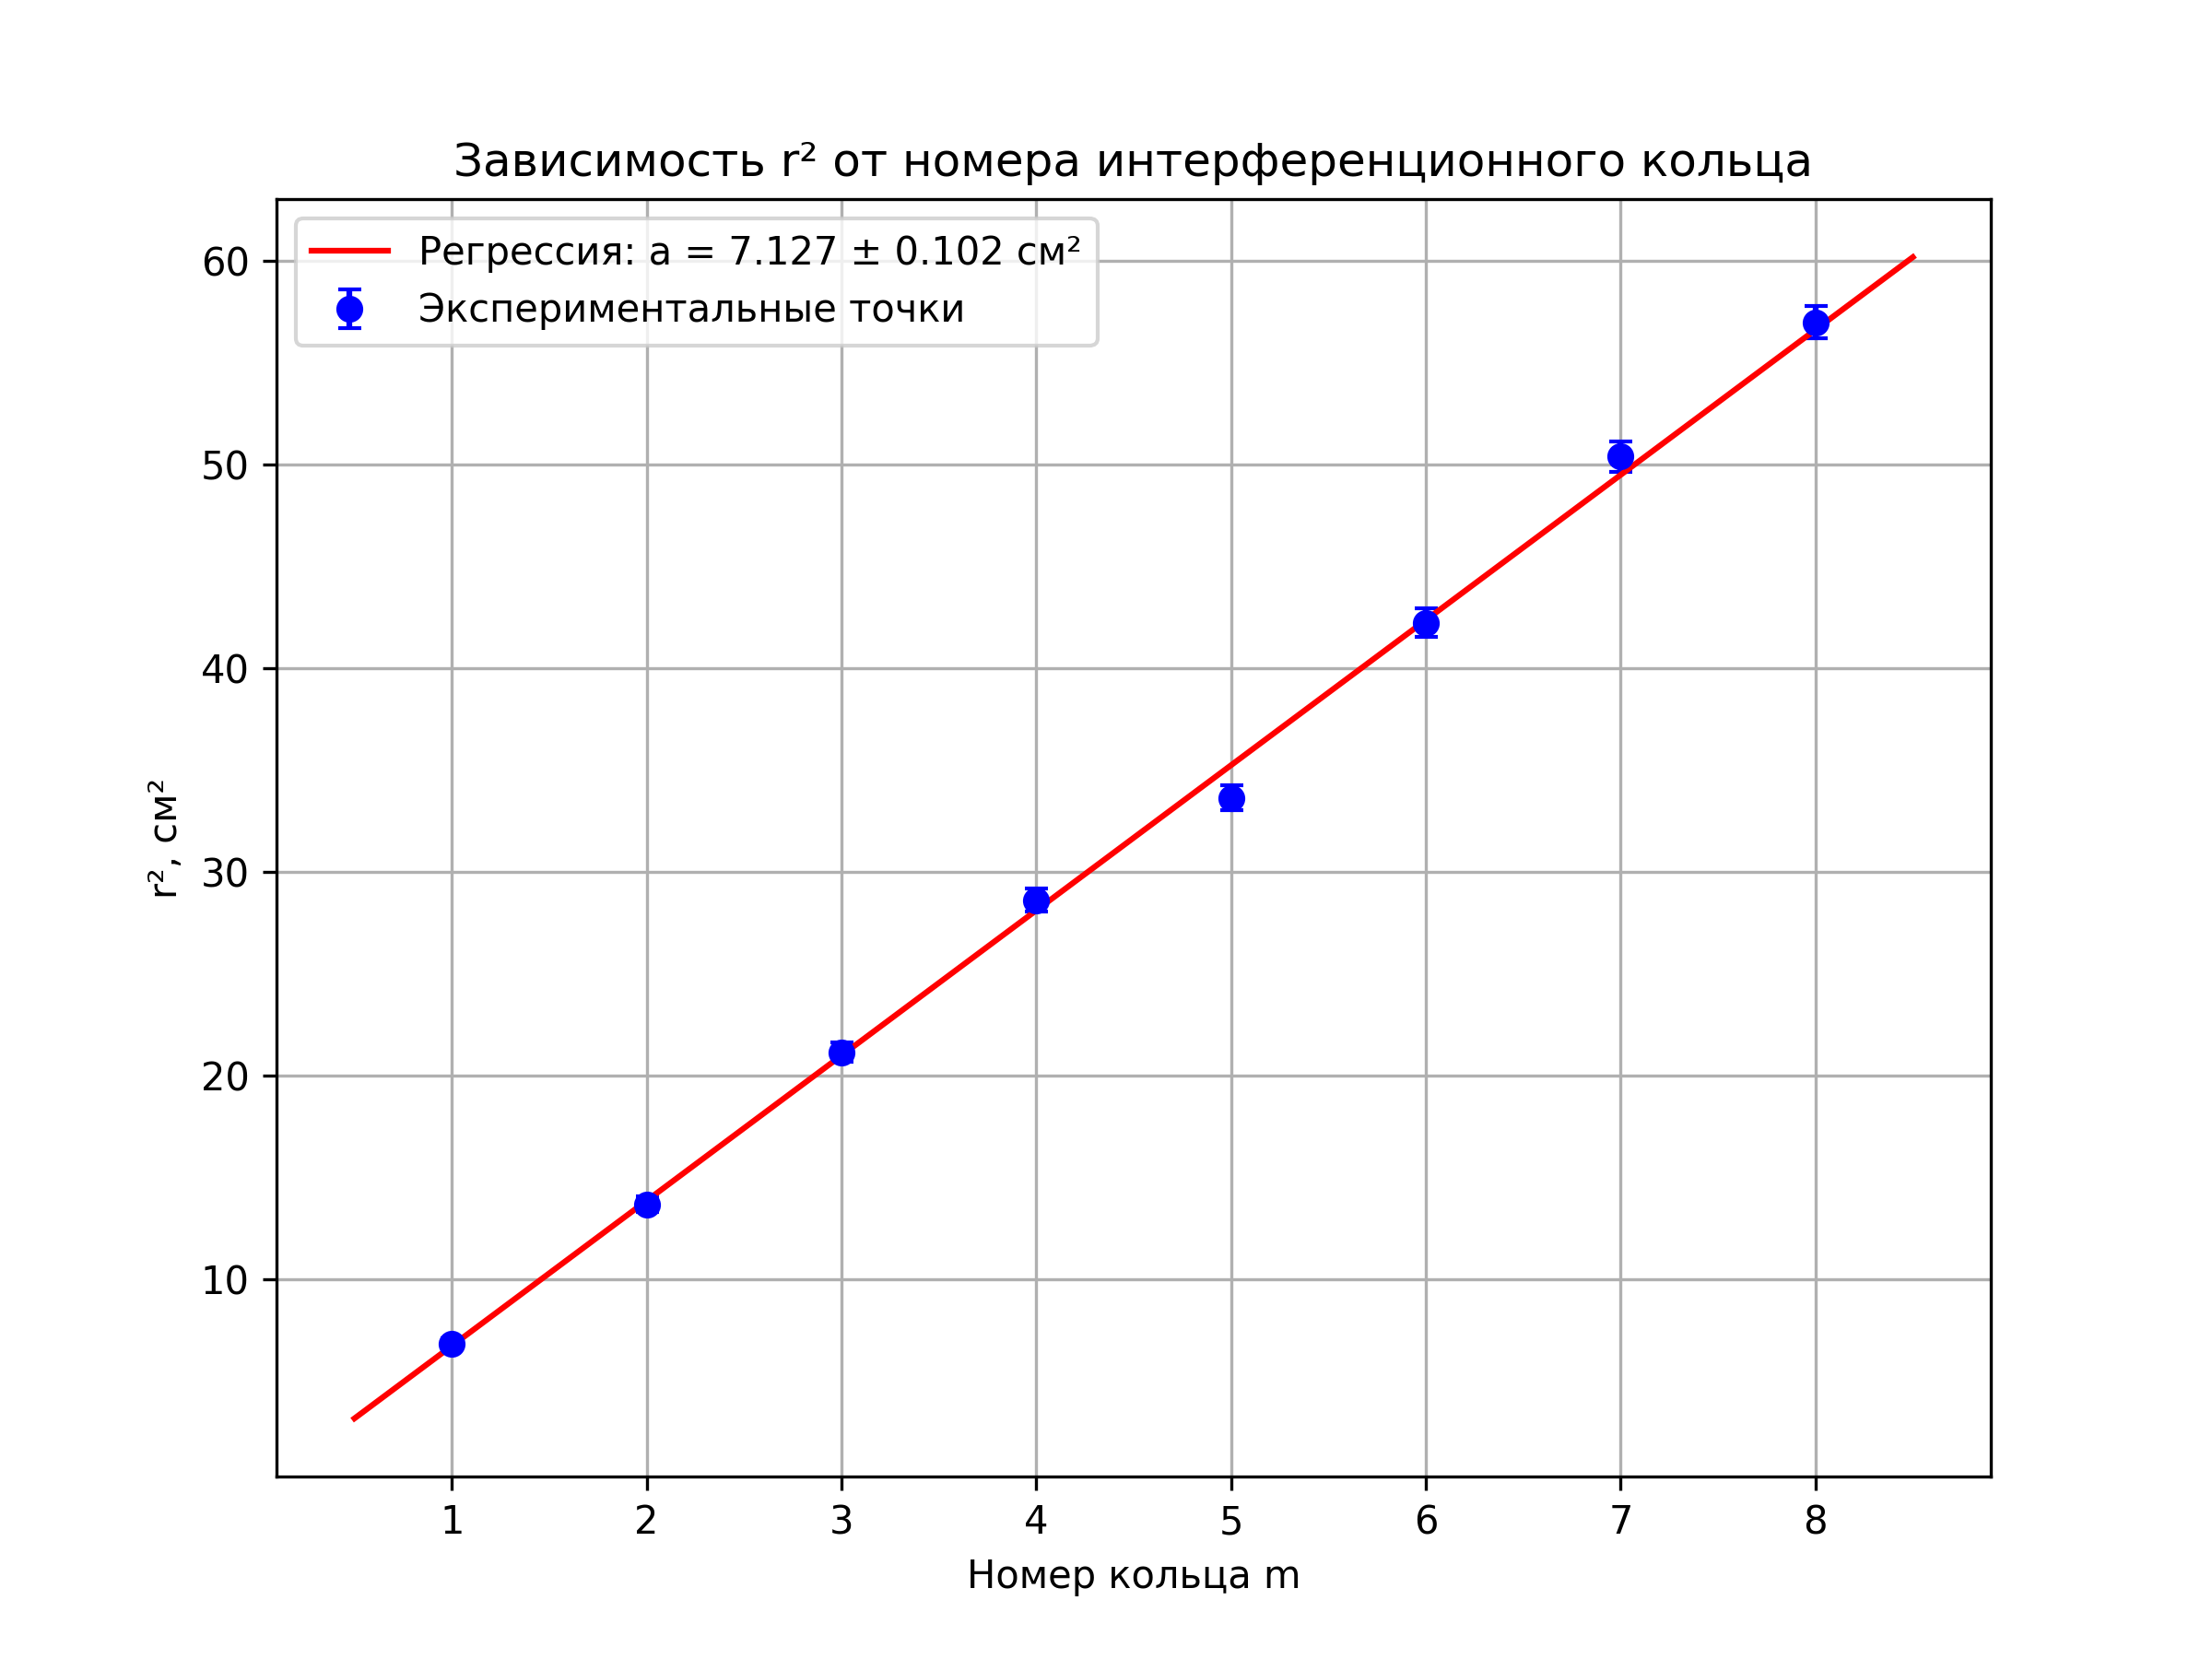
\includegraphics[width=0.7\textwidth]{Graphics/r2_vs_m.png}
    \caption{График 1. Зависимость квадрата радиуса интерференционного кольца от номера.}
\label{fig:r2m}
\end{figure}

Коэффициент наклона $k = 7,127 \pm 0,102 \ \text{см}^2$.

Используя формулу, следующую из теории интерференции в одноосном кристалле,
\[
r_m^2 = \frac{\lambda}{\ell}\,\frac{(n_o L)^2}{n_o - n_e}\,m,
\]
выразим искомую величину:
\[
n_o - n_e = \frac{\lambda}{\ell}\,\frac{(n_o L)^2}{k}.
\]
Подставим $\lambda = 0{,}630 \pm 0,003$\footnotemark[1] мкм, $\ell = 26 \pm 1$ мм, $n_o = 2{,}29 \pm 0,01$\footnotemark[2] , $L = 75,0 \pm 0,5$\footnotemark[3] и вычислим:
\[
n_o - n_e = 0,100 \pm 0,004.
\]
\footnotetext[1]{Погрешность длины волны в техническом описании лазера не указана, утверждается что $\lambda = 0{,}63$ мкм. Длина волны аналогов гелий-неоновых лазеров составляет 0,633 мкм, поэтому погрешность бралась 0,003 мкм.}
\footnotetext[2]{Погрешность указанных в описании к работе величин бралась по последнему разряду}
\footnotetext[3]{Погрешность оценена в 0,5 см, поскольку точнее определить центр кристалла нет возможности и линейка не жесткая, прогибается.}

\subsection*{Определение полуволнового напряжения}

\subsubsection*{Метод с постоянным напряжением}

При скрещенных поляризациях (горизонтальный анализатор) увеличивали напряжение на кристалле и фиксировали значение, соответствующее максимальной яркости пятна на экране. По шкале блока питания это значение составило $30$ делений, что соответствует $U_{\lambda/2} = 450$ В. При дальнейшем увеличении напряжения яркость уменьшалась до минимума при $U_{\lambda} = 64$ деления ($960$ В), что также соответствует $U_{\lambda/2} = 480$ В (полуволновое напряжение, определённое как половина $U_{\lambda}$).

При параллельных поляризациях (анализатор повёрнут на $90^\circ$) минимум яркости наблюдался при $U_{\text{мин}} = 32$ деления ($480$ В), а максимум — при $U_{\text{макс}} = 60$ делений ($900$ В). Для параллельных поляризаций минимум соответствует $U_{\lambda/2}$, поэтому получаем ещё одно значение $480$ В.

Таким образом, из измерений с постоянным напряжением получены следующие значения $U_{\lambda/2}$:
\begin{itemize}
    \item по максимуму при скрещенных поляризациях: $450 \pm 30$ В;
    \item по минимуму при параллельных поляризациях: $480 \pm 30$ В;
    \item по половине $U_{\lambda}$ при скрещенных: $480 \pm 30$ В.
\end{itemize}

\subsection*{Наблюдение круговой поляризации}
Подадим на кристалл напряжение $U = 225 \pm 30$ В. Вращая анализатор, будем наблюдать за яркостью пятна на экране; установим, что она практически не изменяется, что свидетельствует о круговой поляризации излучения на выходе кристалла.

\subsubsection*{Метод с переменным напряжением (фигуры Лиссажу)}

При подаче на кристалл переменного напряжения и наблюдении фигур Лиссажу на осциллографе определили разность напряжений между соседними минимумами (или между минимумом и максимумом) зависимости $I_{\text{вых}}(U)$, которая соответствует $U_{\lambda/2}$. По осциллограммам получили:
\begin{itemize}
    \item $U_{\lambda/2} = 28$ делений ($420 \pm 30$ В);
    \item $U_{\lambda} = 59$ делений ($885 \pm 30$ В), что даёт $U_{\lambda/2} \approx 442{,}5 \pm 30$ В;
    \item $U_{3\lambda/2} = 90$ делений ($1350 \pm 30$ В), что даёт $U_{\lambda/2} \approx 450 \pm 30$ В.
\end{itemize}

\clearpage
\begin{figure}[h]
    \centering
    
\includegraphics[width=0.4\textwidth]{Pictures/1.jpg}
\end{figure}

\begin{figure}[h]
    \centering
    
\includegraphics[width=0.4\textwidth]{Pictures/2.jpg}
\end{figure}
\clearpage
\begin{figure}[h]
    \centering
    
\includegraphics[width=0.4\textwidth]{Pictures/3.jpg}
    \caption{Рис 2. Фигуры Лиссажу}
\end{figure}


\subsubsection*{Окончательное значение}

Все полученные значения $U_{\lambda/2}$ сведём в табл.~\ref{tab:U_half}. Систематическая погрешность каждого измерения обусловлена точностью отсчёта по шкале источника напряжения и составляет $\Delta_{\text{сист}} = \pm 30$ В. Рассчитаем среднее:

\[
\overline{U}  = 453{,}75 \text{ В}.
\]

стандартное отклонение среднего:

\[
\Delta_\text{случ} = 9,44 \text{ В}.
\]

Общую погрешность найдём как квадратичную сумму случайной и систематической составляющих:

\[
\Delta U = \sqrt{\Delta_{\text{случ}}^2 + \Delta_{\text{сист}}^2} \approx \sqrt{9{,}44^2 + 30^2} \approx 31 \text{ В}.
\]

Окончательно принимаем:

\[
U_{\lambda/2} = 454 \pm 31 \text{ В}.
\]

\begin{table}[h!]
\centering
\begin{tabular}{|c|c|}
\hline
Способ определения & $U_{\lambda/2}$, В \\
\hline
Постоянное напряжение, макс (скрещ.) & $450 \pm 30$ \\
Постоянное напряжение, мин (паралл.) & $480 \pm 30$ \\
Постоянное напряжение, $U_\lambda/2$ (скрещ.) & $480 \pm 30$ \\
Фигуры Лиссажу, $U_{\lambda/2}$ & $420 \pm 30$ \\
Фигуры Лиссажу, $U_\lambda/2$ & $442{,}5 \pm 30$ \\
Фигуры Лиссажу, $U_{3\lambda/2}/3$ & $450 \pm 30$ \\
\hline
Среднее & $454 \pm 31$ \\
\hline
\end{tabular}
\caption{Таблица 3. Значения полуволнового напряжения, полученные разными методами}
\label{tab:U_half}
\end{table}

\section{Результаты и обсуждение}

В ходе выполнения работы были получены следующие результаты.

\subsection*{Двулучепреломление кристалла ниобата лития}

По измеренным радиусам интерференционных колец построена зависимость $r^2(m)$ (рис.~\ref{fig:r2m}). Получено значение двулучепреломления:
\[
n_o - n_e = 0,100 \pm 0,004.
\]

Для ниобата лития при длине волны $\lambda = 632,8$ нм разность показателей преломления составляет $n_o - n_e = 0,083$\footnotemark[4]. Полученное в работе значение превышает табличное примерно на $20\%$. Возможные причины расхождения:

\footnotetext[4]{Источник: \url{https://lenlasers.ru/product/linbo3-dvulucheprelomlyayushchij-kristall-niobata-litiya/}, дата обращения 27.03.2026}

\begin{itemize}
    \item \textbf{Погрешность определения расстояния $L$}. Расстояние от кристалла до экрана измерялось гибкой линейкой, что могло внести систематическую ошибку до $0,5$ см. В формуле $L$ входит в квадрате, поэтому относительная погрешность $2\Delta L/L \approx 1,3\%$ даёт вклад в $n_o-n_e$ около $0,001$.
    \item \textbf{Неточное совмещение центра интерференционной картины с лазерным лучом}. Небольшое смещение приводит к неправильному определению $r_m$ и, следовательно, к изменению наклона.
    \item \textbf{Температурная зависимость показателей преломления}. Измерения проводились при комнатной температуре, тогда как табличные значения обычно приведены для $25^\circ$C. Для ниобата лития температурный коэффициент показателя преломления может дать заметную поправку.
\end{itemize}

С учётом вычисленной погрешности $\pm 0,004$ полученное значение $0,100$ не противоречит табличному в пределах $4\sigma$, однако систематическое завышение указывает на присутствие неучтённых факторов, прежде всего погрешности в определении $L$.

\subsection*{Полуволновое напряжение}

Полуволновое напряжение определялось двумя независимыми методами: по изменению интенсивности при постоянном напряжении и по фигурам Лиссажу при переменном напряжении. Результаты сведены в табл.~\ref{tab:U_half}.

Разброс отдельных значений составляет от $420$ до $480$ В, что соответствует относительному разбросу $\sim 13\%$. Систематическая погрешность отсчёта по шкале источника ($\pm 30$ В) вносит основной вклад в итоговую погрешность. Среднее значение $U_{\lambda/2} = 454 \pm 31$ В.

Следует отметить, что значения, полученные по фигурам Лиссажу ($420$ В, $442,5$ В, $450$ В), систематически немного ниже определённых при постоянном напряжении ($450$–$480$ В). Это может быть связано с гистерезисом или остаточной поляризацией кристалла при работе на постоянном напряжении, а также с неточностью визуального определения максимума/минимума интенсивности.

\subsection*{Круговая поляризация}

При подаче напряжения $U = 225 \pm 30$ В (что соответствует половине среднего $U_{\lambda/2}$) вращение анализатора не приводило к изменению яркости пятна. Это подтверждает, что на выходе кристалла формируется свет с круговой поляризацией, что полностью соответствует теории: при сдвиге фаз $\Delta\varphi = \pi/2$ между ортогональными компонентами поляризации линейно поляризованный на входе свет превращается в циркулярно поляризованный.

\subsection*{Фигуры Лиссажу}

Наблюдавшиеся на осциллографе фигуры Лиссажу при скрещенных поляризациях имели вид, описываемый функцией $\sin^2(\frac{\pi}{2}\frac{U}{U_{\lambda/2}})$, что соответствует теоретической зависимости (3). При переходе к параллельным поляризациям форма фигур изменялась на $\cos^2(\frac{\pi}{2}\frac{U}{U_{\lambda/2}})$, что также согласуется с теорией.

\section{Выводы}

В результате выполнения лабораторной работы:

\begin{enumerate}
    \item Проведена юстировка оптической схемы, получена чёткая интерференционная картина (коноскопические кольца) от кристалла ниобата лития.
    \item По радиусам интерференционных колец определено двулучепреломление кристалла: $n_o - n_e = 0,100 \pm 0,004$.
    \item Исследован линейный электрооптический эффект (эффект Поккельса) в поперечной геометрии. Экспериментально установлено полуволновое напряжение $U_{\lambda/2} = 454 \pm 31$ В
    \item Показано, что при напряжении $U = U_{\lambda/2}/2$ на выходе кристалла формируется свет с круговой поляризацией.
    \item Методом фигур Лиссажу подтверждена синусоидальная зависимость интенсивности прошедшего света от приложенного напряжения при скрещенных поляризациях и косинусоидальная — при параллельных.
\end{enumerate}

Все поставленные цели работы достигнуты; полученные результаты удовлетворительно согласуются с теорией в пределах экспериментальных погрешностей.

\end{document}